\chapter{Realer Demonstrator}  
\label{ch:realer demonstrator}
In diesem Kapitel werden die nötigen Punkte zum Übergang auf den Demonstrator angesprochen. Dazu gehören die Messungen von Maximalgeschwindigkeiten, die Bildverarbeitung, Sicherheitsvorkehrungen um Kollision und Schaden zu verhindern und ein Benutzerinterface für den Bedierner des Demonstrators. Alle Bildverarbeitungsschritte wurden in Python mit der OpenCV Bibliothek durchgeführt.

\section{Geschwindigkeitsmessungen}
\label{sect:geschwindigkeitsmessungen}

Bei den Geschwindigkeitsmessungen wurden die Maximalgeschwindigkeit von Roboter und Puck gemessen. Während die Maximalgeschwindigkeit des Roboters relativ einfach erreicht werden kann ist die des Pucks abhänig vom Spieler. Unsere Messung wurde deshalb an einem Schuss durchgeführt, denn wir nach bestem Gewissen als ausreichend schnell bewerten würden. Gemessen wurde anhand von Videomaterial der Kamera. Mit dem Programm Tracker des Open Source Physics Projekts \cite{tracker} wurde das Material analysier. Diese Software erlaubt es einen Punkt (Puck oder Roboter) von Frame zu Frame zu verfolgen. Mit der Bildwiederholungsrate und einem Maßstab können nun Werte ermittelt werden. Da diese Werte für das Training in der Softwareumgebung von Nöten ist wurde als Maßstab nicht die Abmessung in Metern des realen Demonstrators genutzt sondern die Länge in Unitylängeneinheiten. Die Ergebnisse sind wie folgt ausgefallen:\\
\begin{figure}
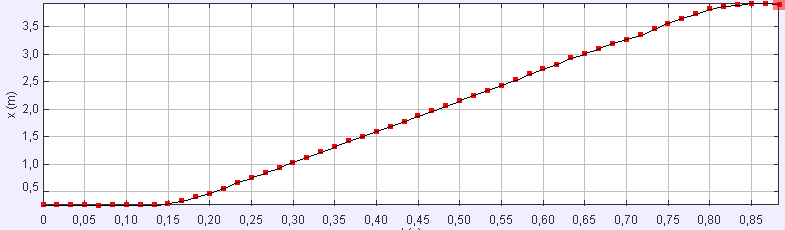
\includegraphics[width=\textwidth]{images/messung_robo_x}
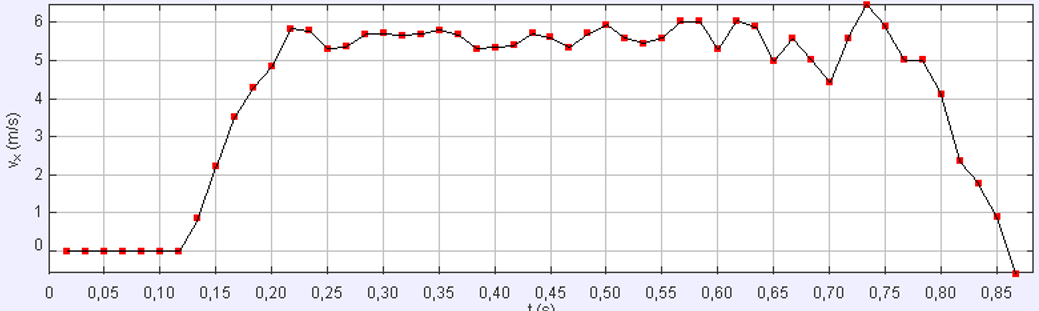
\includegraphics[width=\textwidth]{images/messung_robo_v}
 \caption{Messwerte des Roboters }
 \label{mess_robo}

Das obere Diagramm in Abbildung \ref{mess_robo} zeigt den zurückgelegten Weg des Roboters über die verstrichene Zeit seit Beginn der Messung. Das untere zeigt den Geschwindigkeitsverlauf über die Zeit. Die Maximalgeschwindigkeit ist also in etwa 6m/s. Da im Wegdiagramm in sehr guter Näherung eine Gerade während der Bewegung zu sehen ist kann die Geschwindigkeit während dieser Zeit als konstant angenommen werden. Rechnent man die Durchschnittsgeschwindigkeit über den Zeitraum von 0.2 bis 0.75 Sekunden aus so erhält man bei einem zurückgelegten Weg von 3.2 (LE)Längenenheiten eine Geschwindigkeit von 5.8 LE/s. Nach Rundung wurde mit dem Wert 6 LE/s traininiert.
\end{figure}

\begin{figure}
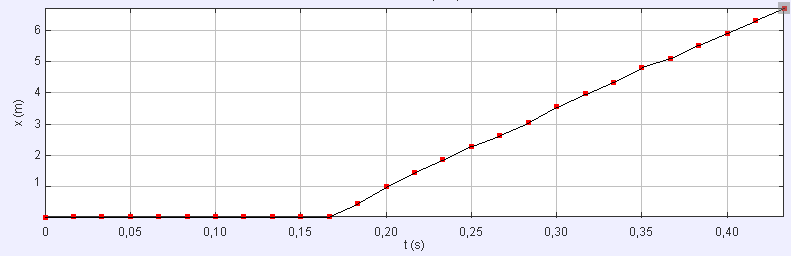
\includegraphics[width=\textwidth]{images/messung_bolzen_x}
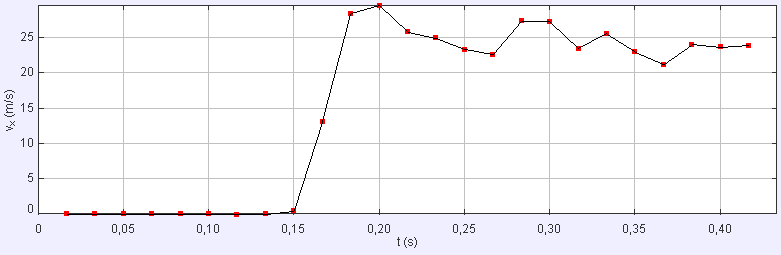
\includegraphics[width=\textwidth]{images/messung_bolzen_v}
 \caption{Messwerte des Pucks}
 \label{mess_puck}
Diese Diagramme sind von der Messung der Bewegung des Pucks. Auch hier zeigt da obere den Verlauf des zurückgelegten Weges und das untere den Geschwindigkeitserlauf über die Zeit. Rechnet man hier die Steigung der Geraden im Wegdiagramm mit einer Wegdifferenz von 6.8 LE und einer verstrichenen Zeit von 0.33 Sekunden aus, so ergibt sich ein Wert von 20.6 LE/s. Da die Puckgeschwindigkeit bei anderen Spielern noch höher sein könnte wurde für die Simulation in Unity und damit auch für die Trainings eine Maximalgeschwindigkeit des Pucks von 25 LE/s angenommen. 
\end{figure}

\clearpage
\begin{figure}
\section{Benutzeroberfläche}
\label{sect:gui}
Das graphical use interface (GUI) wurde in Python geschrieben. Die Bibliothek Tkinter wurde dabei genutzt. Diese Bibliothek wurde unter einer Pythonlizenz veröffentlicht und ist so frei für alle zugänglich. Dadurch ist der Einsatz der GUI in jedem Fall rechtlich unbedenklich.\\

\subsection{Ansicht der Oberfläche}
\label{subsect:gui_pic}


Die Folgende Abbildung zeigt das Interface. Die markierten Bereiche und Elemente werden im Folgenden erklärt.\\
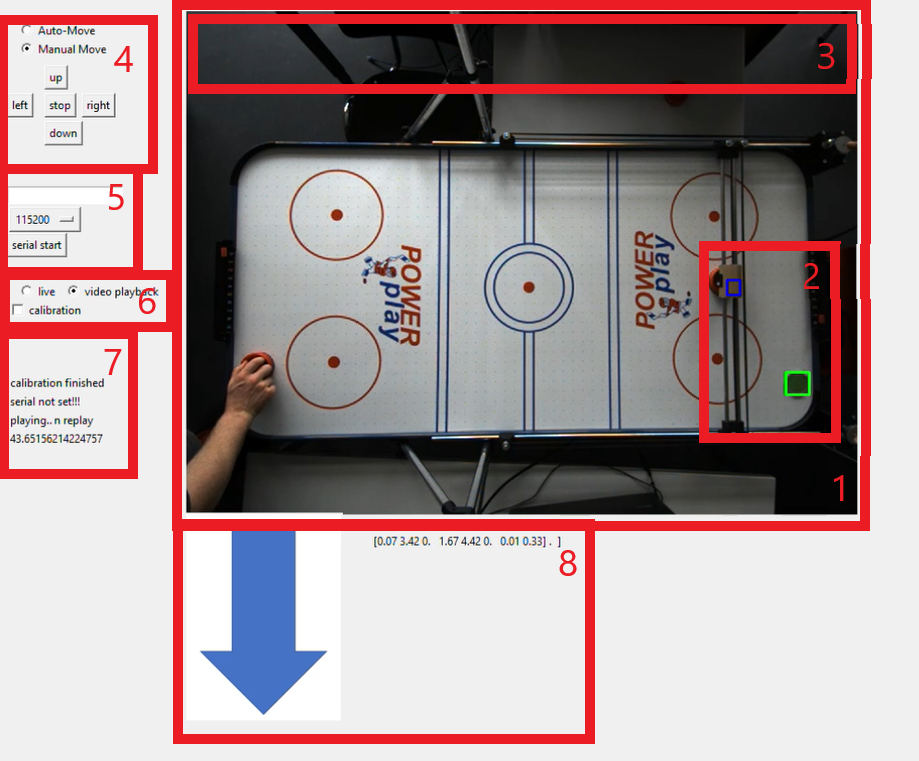
\includegraphics[width=\textwidth]{images/gui_pic_marked}
 \caption{Benutzeroberfläche}
 \label{gui_pic}

\end{figure}
\begin{figure}
1:\\
Hier ist das Kamerabild oder eine Videosequenz zu sehen. Das Bild wird wird, je nach Zustand, um einige Informationen ergänzt.\\
2:\\
Eine Ergänzung zum Kamerabild ist die Markierung von Roboter und Puck sofern sie erkannt wurden. Der Puck wird mit einem grünen und der Roboter mit einem blauen Rechteck markiert.
\\
3:\\
In diesem Bereich wird eine Meldung gegeben wenn, wenn Puck oder Robote nicht erkannt werden.\\
4:\\
In diesem Bereich sind die Bedienelemente für das manuelle Verfahren. Mit den beiden Knöpfen kann eine Auswahl zwischen einem autonomen Bewegungsmodus (Auto-Move) und dem manuellen Verfahrmodus gemacht werden. Ist der manuelle Modus ausgewählt kann mit den darunter liegenden Feldern der Roboter bewegt werden. Im Auto-Move Modus obliegt die Entscheidung sich zu bewegen dem Agenten. Der Agent kann im Gegensatz zum manuellen Modus auch diagonal verfahren. \\
5:\\
Hier kann die serielle Kommunikation gesteuert werden. Im Eingabefenste muss der Port eingegeben werden (z.B. COM4). Darunter ist ein Drop-Down Menü, in dem die Baudrate gewählt werden kann. Mit dem Knopf serial start wird die Kommunikation aufgebaut. Besteht schon eine wird die alte erst beendet bevor eine neue aufgebaut wird.\\
6:\\
Im diesem Ausschnitt kann die Videoquelle gewählt werden. Bei live wird auf das aktuelle Kamerabild zugegriffen, bei video playback kann eine Aufnahme genutzt werden. Das ist besonders nützlich wenn zuhause am Schribtisch  am Projekt gearbeitet werden muss und man unabhänig vom Zugang zum Airhockey-Tisch sein will. In der kleinen Box darunter kann der Kalibrierungsmodus initialilisiert werden. Die Box bleibt dann ausgewählt bis die  Kalibrierung erfolgreich abgeschlossen wurde.\\
7:\\
In diesem Bereich werden nur Statusmeldungen gemacht. Er enthält keine Bedienelemente. Die erste Zeile gibt Aufschluss über den Status der Kalibrierung. Die zweite informiert über die serielle Kommunikation. Die dritte enthält eine Aussage über den Spielmodus. In der letzten wird angegeben, mit welcher Frequenz die ganze Anwendung läuft.\\
8:\\
Hier sind Eingang und Ausgang des neuronalen Netzwerkes angegeben. Der Vektor enthält die Informationen zum Spielgeschehen aus der Bildverarbeitung und der Pfeil zeigt das Ergebniss der Interferenz an. 
\end{figure}
\clearpage

\subsection{Programmablauf der GUI-Anwendung}
\label{subsect:pap}

In diesem Abschnitt wird der Ablauf der einzelnen programmtechischen Schritte erklärt. Zu beachten ist dabei, dass zwei Prozess parallel ablaufen müssen. Das liegt daran, dass das Interface kontinuierlich überwacht und auf Eingaben überprüft werden muss. Gleichzeitig müssen die anderen Vorgänge zur Bildverarbeitung, zur Kommunikation etc. ablaufen. 
Der Prozess für die Funktion der Oberfläche und der Prozess für den standartmäßigen Ablauf sind also immer aktiv, beziehungsweise laufen in einer Schleife und werden koninuierlich wiederholt. Wenn eine Benutzerinteraktion ausgelöst wird, wird diese in die Schleife der  Interfacefunktion oder der Standartabläufe eingefügt. Wird beispielsweiße ein Haken in der Box zur Kalibrierung erfasst ändert das den Standartablauf, wird der Knopf für die serielle Kommunikation gedrückt verlängert das die Schleife des Interfaces. Alle Funktionen, die direkt durch ein Bedienelement hervorgerufen weden verlängern die Interfaceschleife, der Rest, bei dem nur ein Parameter angepasst wird, wird während des Standartablaufen abgearbeitet.\\
 Funktionen der Interfaceschleife sind:\\
\begin{itemize}
\item manuelle Bewegung
\item Start der seriellen Kommunikation
\item Wechsel der Videoquelle
\end{itemize}

Wie die anderen Funktionen abgearbeitet werden ist in der Abbildung \ref{gui_pap} dargestellt. Im Ablaufgraphen stelle die grünen Rechtecke Programmschritte dar. Habe die Rechtecke links und rechts einen Doppelstrich bedeutet das, dass diese Prozesse komplexer sind und noch genauer erläutert werde. Die orangenen Rauten stehen für eine Entscheidung. Die Sechsecke stellen Anfang und Ende der Schleife dar.\\\\

Zu Beginn des Programms wird die Viualisierung erstellt. Dazu wird ein Objekt der Klasse Window angelegt. Dieses hat durch Vererbung aus der Tkinter Bibliothek die nötigen Methoden und Attribute um das Fenster mit der mainloop Methode zu erstellen und die beiden Schleifen zu starten. \\
Im Standartablauf wird als erstes überprüft, ob schon eine Videoquelle festgelegt wurde. Ist das nicht der Fall, so ist der Durchlauf der Schleife schon vorbei. \\
Als nächstes wird geprüft, ob eine Kalibrierung durchgeführt werden soll. Ist das der Fall wird ein Kalibrierungsversuch unternommen. Scheitert dieser, so wird sofort zum Update des Interfacebildes gesprungen. Ist er erfolgreich so kann der Standartablauf weiter verfolgt werden.\\
Die nächste Abfrage ist, ob schon kalibriert wurde. Das ist wichtig, denn es besteht auch die Möglichkeit, dass noch nicht kalibriert wurde und der Haken im Interface noch nicht gesetzt wurde.\\
Nun erfolgt der Schritt, bei dem die Input Daten für den Agenten aus dem Kamerabild ermittelt werden.\\
Wenn Puck und Roboter erkannt werden kommt es zu Spielen. Dabei wird die Ausgabe des Netzwerkes nach einer Sicherheitsüberprüfung ausgeführt.\\
Ist es der Fall das nur der Roboter erkannt wird ist davon auszugehen, dass der Puck nicht im Spiel ist. Dann wird der Roboter in eine Ausgangsposition mittig vor dem Tor fahren und auf die Fortsetzung des Spiels warten.\\
Da es durchaus vorkommen kann, dass durch die Lichtverhältnisse oder Ähnlichen für ein oder zwei Einzelbilder nicht Puck und Roboter erkannt werden obwohl beide am Tisch sind wird in diesem Fall der letzte Bewegungsbefehl wiederholt. Dazu wird überprüft, wie lange die Berechnung des letzten Befehls zurück liegt. Ist er zu alt wird in die Ausgangsposition verfahren.\\
Wenn der Roboter zu lange nicht mehr erkannt wurde wird jede Bewegung verhindert um eine Kollision zu verhindern. Dabei ist es egal ob der Puck noch detektiert wird.\\
Als letzter Punkt der Schleife steht das Update des Bilds für das Interface. Das erfolgt immer, außer es gibt keine Videoquelle.\\ 




\begin{figure}[h]
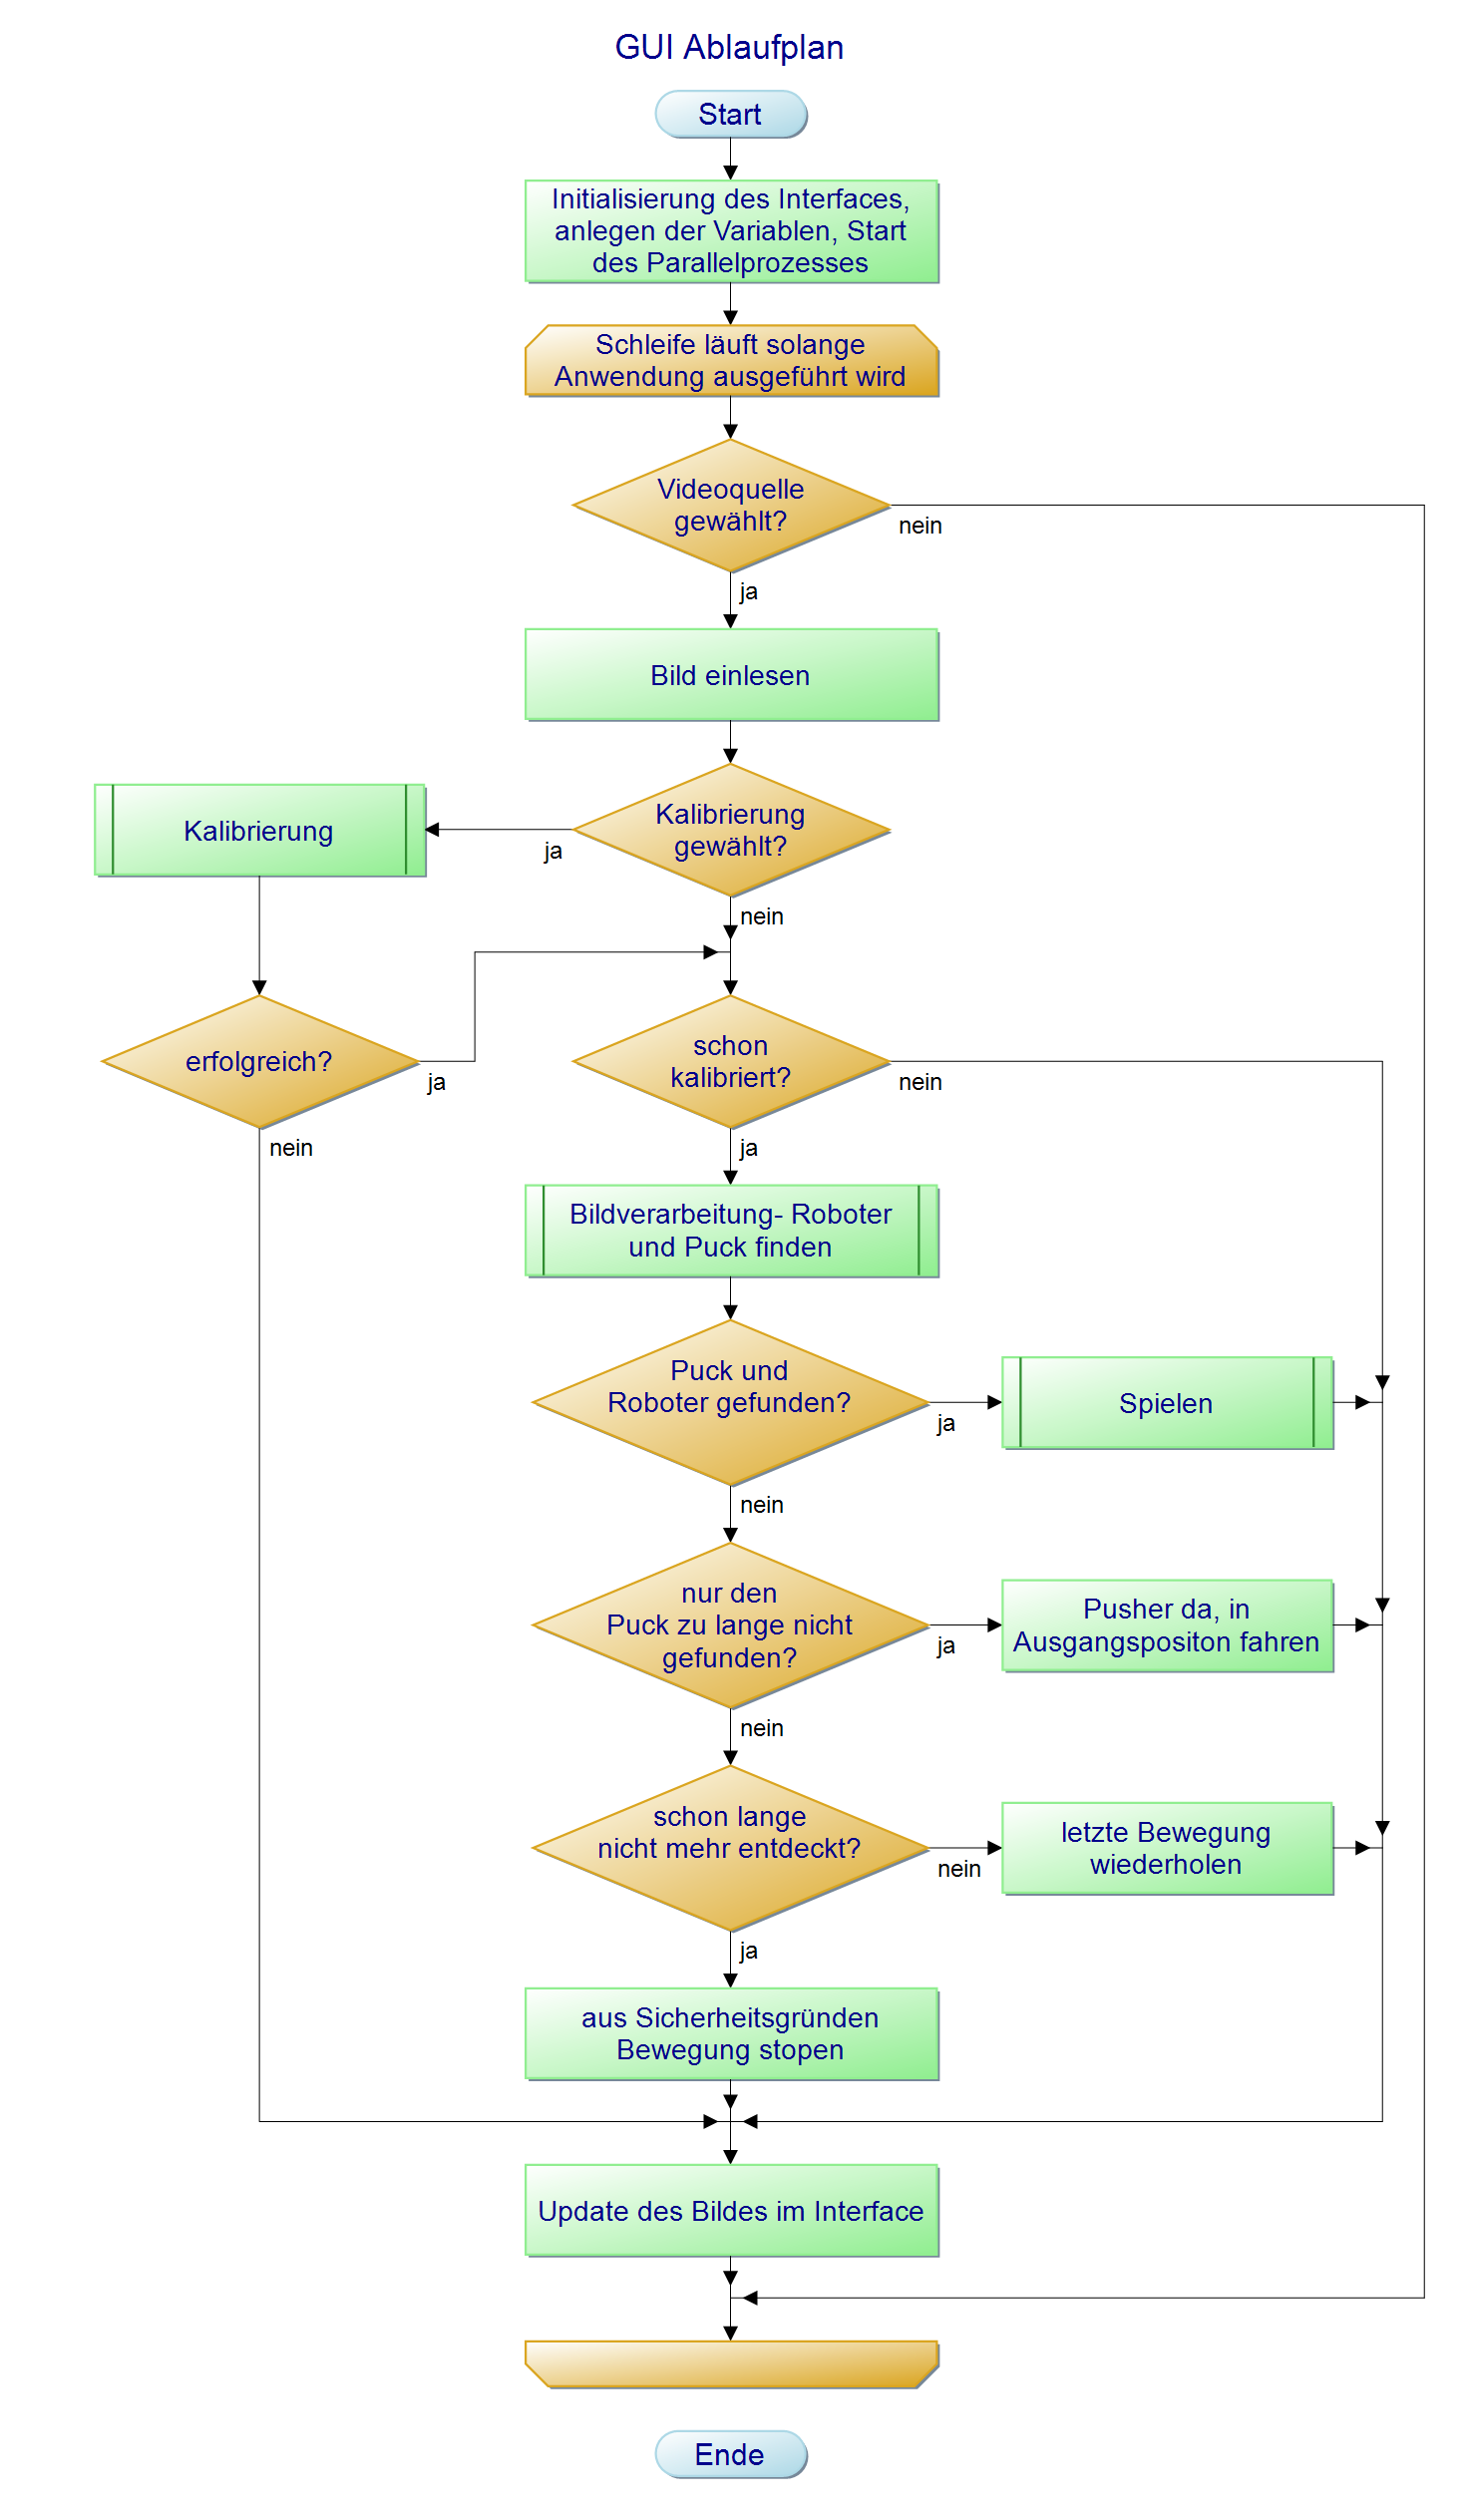
\includegraphics[scale =0.3]{images/gui_pap}
 \caption{Programmablaufplan des Standartablaufes}
 \label{gui_pap}

\end{figure}

\clearpage


\section{Kalibrierung}
\label{sect:kalib}
Bei der Kalibrierung geht es darum das Spielfeld vor der Kamera zu vermessen und auf das Spielfeld in der Unity Umgebung zu Übertragen. Das ist wichtig, da der Agent in der Softwareumgebung traininiert wurde und dem entsprechend auch Größen in Unity Längeneinheiten angegeben werden müssen. Angaben in Metern oder Pixeln müssen also umgerechnet werden. Da wir davon ausgehen können, dass die Kamera senkrecht über dem Spielfeld hängt und andere Verzerrungseffekte vernachlässigbar sind, können wir das Problem zweidimensional betrachten. Das bedeutet, dass die Felder zueinander verdreht um die Z-Achse, verschoben um die X- und Y-Achse und scaliert entlang der X- und Y-Achse sind. Eine Verkippung um die X- und Y-Achsen sowie eine Verschiebung in Z-Richtung fallen weg. \\
Um all diese Parameter berechnen zu können müssen auf dem realen Spielfeld mindestens drei Punkte ihrem Gegenstück aus der Unity Version zugeordnet werden.\\
Als markante Punkte haben wir die vier roten Kreise auf dem Spielfeld gewählt. Um diese auf dem Kamerabild zu erfassen muss zuerst ein bestimmter Farbberich extrahiert werden.Dazu wird das Ausgangsbild in den HSV-Farbraum überführt. Statt der Farbwerte für die Kanäle rot grün und blau sind Farben nun in durch die Kategorien Hue (Farbwert), Saturation (Reinheit, Sattigkeit), und Value (Helligkeit) beschrieben. Da eine Verstärkung der Beleuchtung nun nur noch eine Änderung am V-Wert (Value) zur Folge hat wird die Seperation eines Objekts dadurch viel stabiler.\\

\begin{figure} [h]
\begin{minipage}[t]{0.5\textwidth}
\vspace{0pt}

Nachdem der gewünschte vordefinierte Farbraum herausgefiltert wurde bleibt ein Binärbild, in dem alle Pixel die im Orginalbild in den Farbraum fallen, weiß sind. Mit hilfe der in OpenCV implementierten HoughCircles Funktion \cite{rhody2005lecture} können nun die Mittelpunkte der Kreise bestimmt werden. Dazu ist von Vorteil, dass die Größe vorher schon relativ genau bekannt ist. \\ 
Die Mittelpunkte werden danach mit vorher festgelegten Berichen abgeglichen. Da die Kamera fest moniert ist sollte nun klar sein, ob ein Kreis links oben, rechts oben, links unten oder rechts unten ist. Gibt es midestens drei Übereinstimmungen kann der Mittelpunkt des Spielfeldes und die Ausrichtung sowie die Skalierung relativ zum Unityfeld ermittelt werden. Mit diesem Wissen kann nun mittels zweier Funktionen die Umrechnung von realen in Unitykoordinaten und umgekehrt durchgeführt werden.\\
 Im Vergleich zum Programmablaufplan in der Abbildung \ref{gui_pap} ist der aus Abbildung \ref{kalib_pap} deutlich überschaubarer. Er ist bis auf eine Verzweigung geradlinig.
\end{minipage}
\hspace{0.1\textwidth}
\begin{minipage}[t]{0.3\textwidth}
\vspace{0pt}
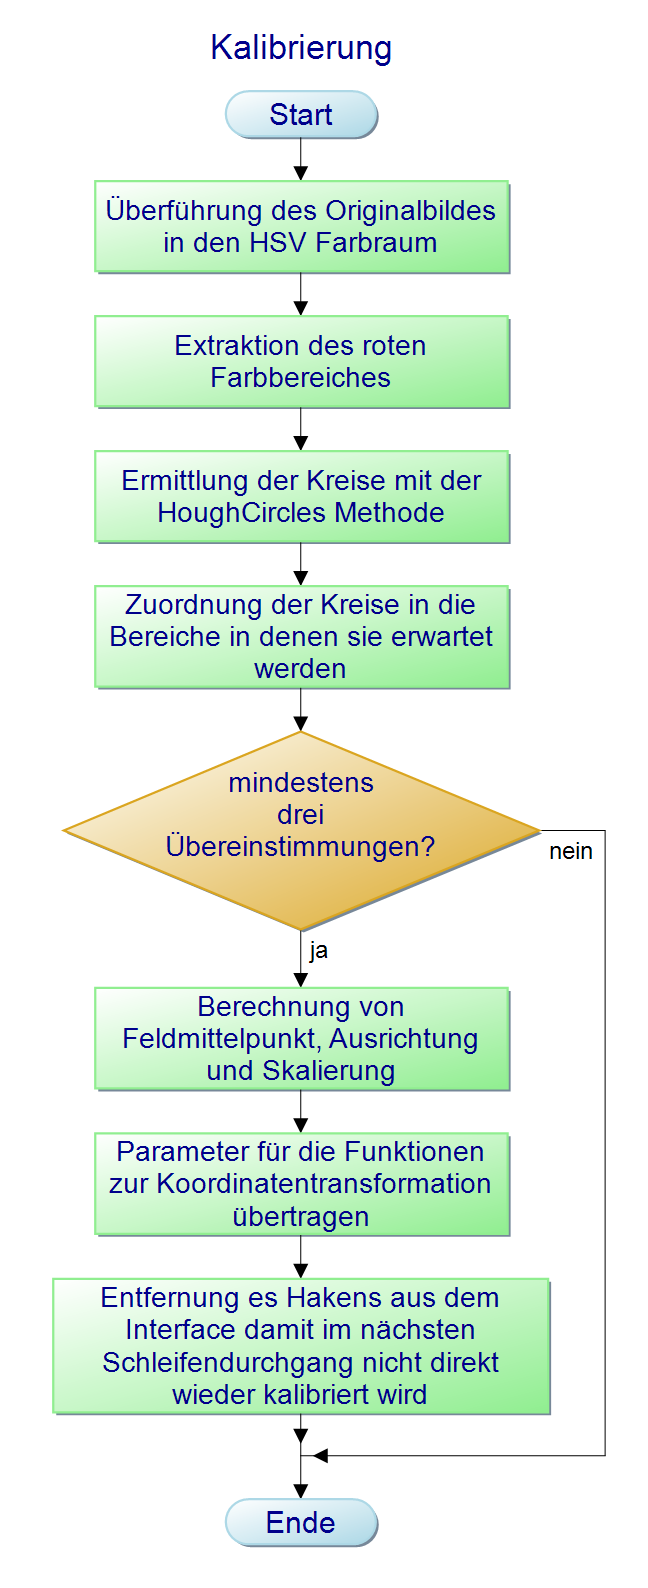
\includegraphics[scale =0.3]{images/kalibrierung_pap}
 \caption{Programmablaufplan der Kalibrierung}
 \label{kalib_pap}
\end{minipage}
\end{figure}

\begin{figure} [h]
\begin{minipage}[t]{0.4\textwidth}
\vspace{0pt}
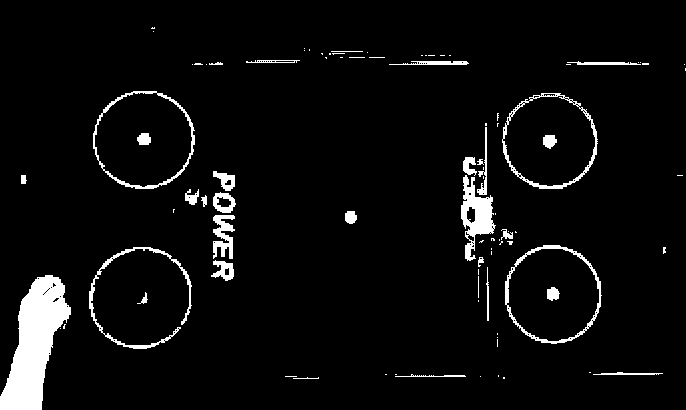
\includegraphics[scale =0.3]{images/kalib_bin}


\end{minipage}
\hspace{0.1\textwidth}
\begin{minipage}[t]{0.4\textwidth}
\vspace{0pt}
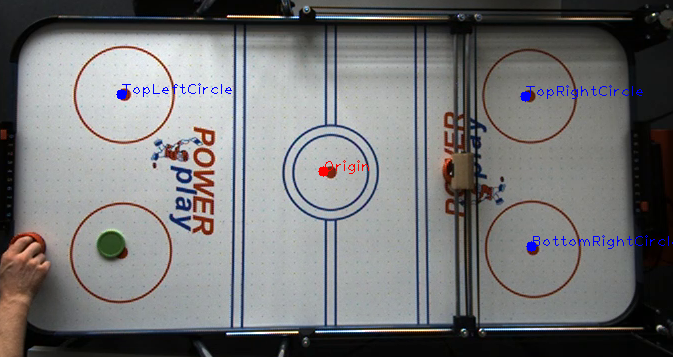
\includegraphics[scale =0.3]{images/kalib_circ}

\end{minipage}
 \caption{Zwischenergebnisse der Kalibrierung}
 \label{kalib_process}
\vspace{5pt}

Das linke Bild das Binärbild, das entsteht wenn nur ein bestimmter Farbbereich gewählt wird. Neben den Kreisen wird auch ein Teil der Schrift und der Arm des menschlichen Spielers mit binarisiert. Nach der HoughCircles Methode und der Zuordnung kann der Mittelpunkt des Spielfelds, wie man auf der rechten Seite erkennen kann ziemlich gut ermittelt werden.
\end{figure}

\clearpage
\section{Puck und Robotererkennung}
\label{sect:puck_robo_erk}
Um am realen Demonstrator den Agenten aus der Simulation nutzen zu können müssen alle Eingabewerte die während des Trainings von Unity bereitgestellt wurden hier anders ermittelt werden. Da viele Sensoren teuer und aufwändig zu implementieren sind haben wir uns entschlossen alle Daten aus den Kamerabildern zu beziehen. Die benötigten Daten sind Position des Pucks, Geschwindigkeit des Pucks und Position des Roboters. Alle drei Daten sind als X- und Y-Wertepaar nötig. Wie diese Imformationen erlangt werden soll in den folgen Abschnitten klar werden.\\


\begin{figure} [h]
\begin{minipage}[t]{0.35\textwidth}
\vspace{0pt}
Grundlage der Bildverarbeitung ist auch hier die Extaktion bestimmter Farbbereiche. Zuerst wird dazu wieder in den HSV- Raum übergegangen um dann ein Binärbild mit den erwünschten Bereichen in weiß zu erhalten. Da hier nicht mit der HoughCircles Funktion schnell ein Ergebniss erreicht werden kann wir danach eine kleine Errosion durchgeführt um das Binärbild übersichtlicher zu machen. Nach dieser Errosion sollten kaum mehr weiße Flecken außer der gewünschten Kontur übrig sein. Aus den verbleibenden Konturen wird dann die größte herausgesucht. Passt ihre Größe zu der des gesuchte Objekts (Puck oder Roboter) wird ihre Positon ermittelt. Hierzu werden die vorkalibrierten Funktionen verwendet. Im Unity Koordinatensystem sind die Werte dann geeignet für den Agenten. Aus der aktuellen Position, der letzen Position und der verstrichenen Zeit wird dann noch die Geschwindigkeit berechnent. 

\end{minipage}
\hspace{0.1\textwidth}
\begin{minipage}[t]{0.45\textwidth}
\vspace{0pt}
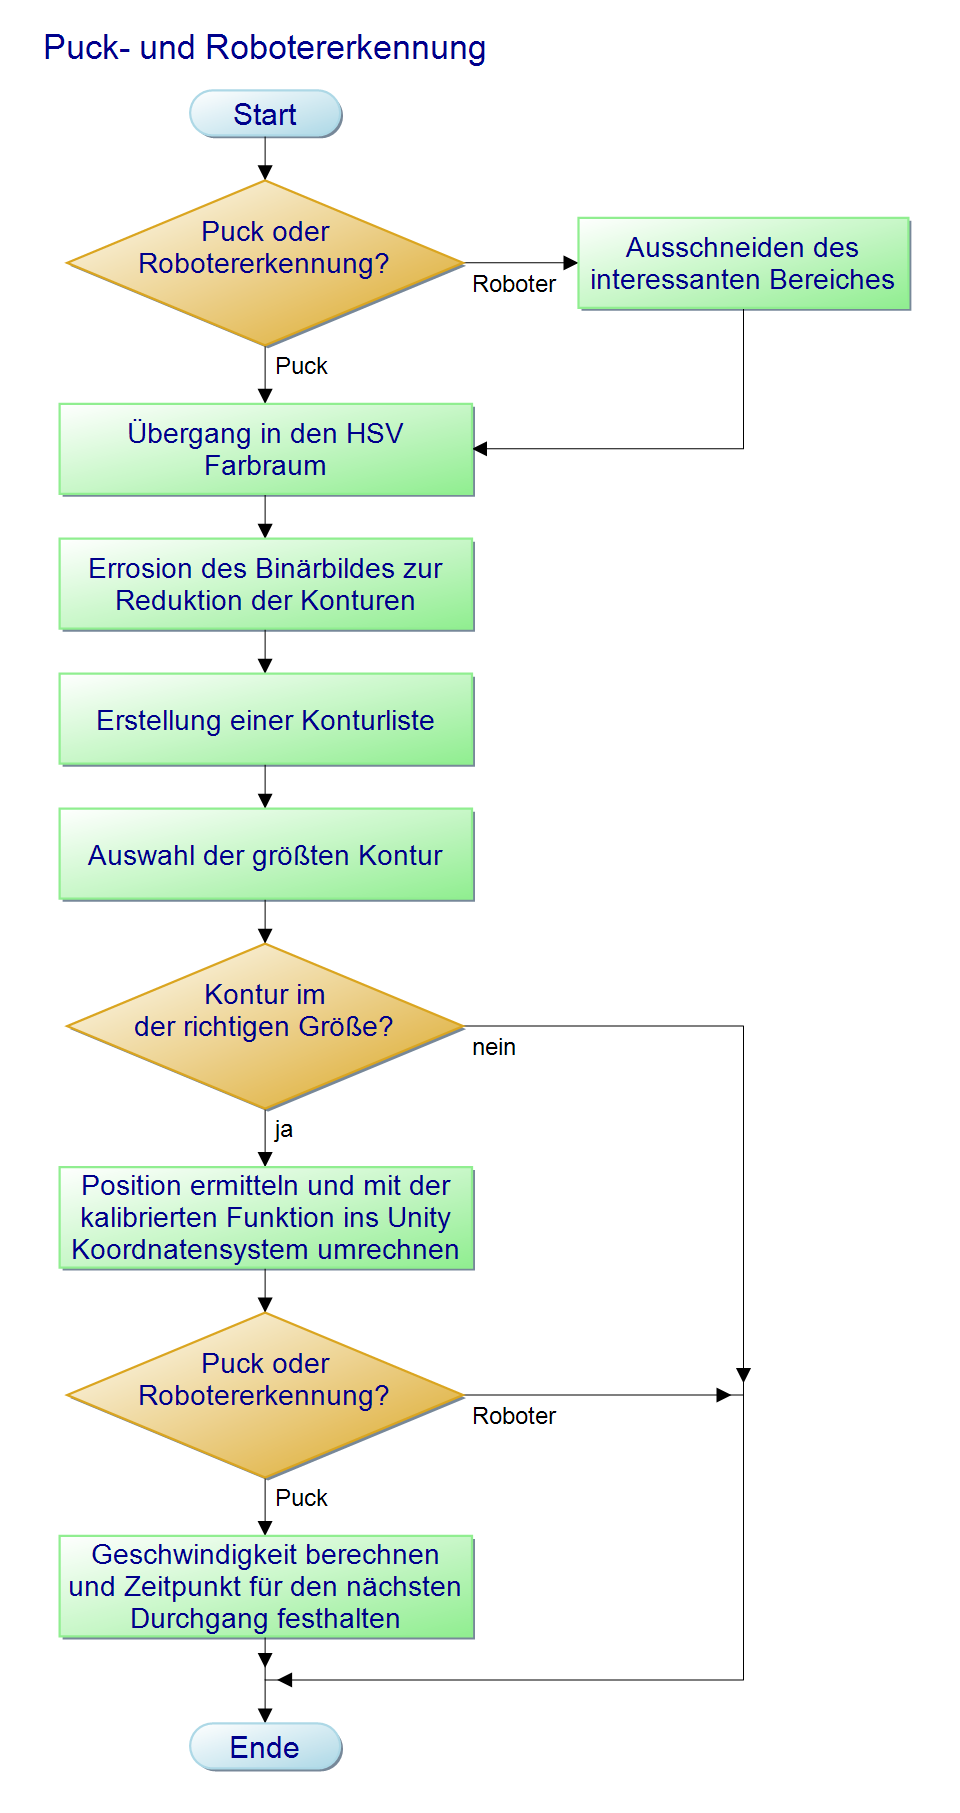
\includegraphics[scale =0.3]{images/bv_pap}
 \caption{Programmablaufplan der Puck- und Robotererkennung}
 \label{bv_pap}
\end{minipage}
\end{figure}

Der Vorgang ist bei Puck und Roboter vergleichbar. Die Hauptunterschiede sind die unterschiedlichen Farbräume, der Roboter kann sich nur in seiner Hälfte aufahlten und die Geschwindigkeit ist nur für den Puck zu berechnen. Zwar gibt es noch weitere kleine Unterschiede, beispielsweise bei der Errosion, aber bei beiden Erkennungen wird nach dem gleichen Plan verfahren.

\begin{figure} [h]
\begin{minipage}[t]{0.25\textwidth}
\vspace{0pt}
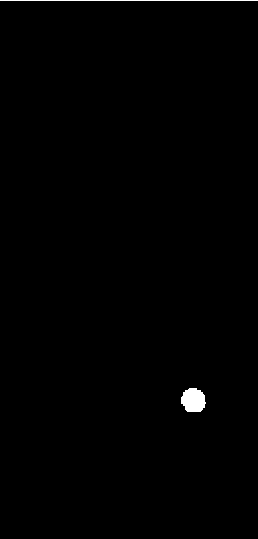
\includegraphics[scale =0.45]{images/bin_puck}
\end{minipage}
\hspace{0.05\textwidth}
\begin{minipage}[t]{0.25\textwidth}
\vspace{0pt}
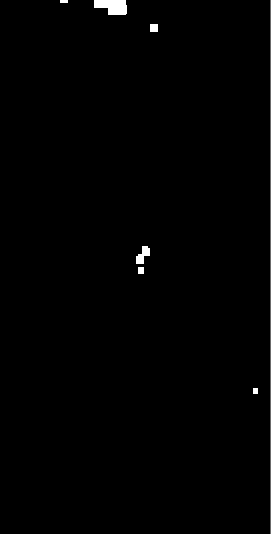
\includegraphics[scale =0.45]{images/bin_robo}
\end{minipage}
\hspace{0.05\textwidth}
\begin{minipage}[t]{0.25\textwidth}
\vspace{0pt}
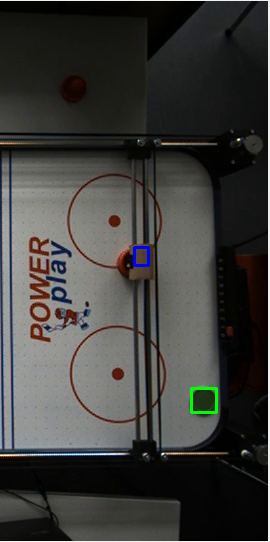
\includegraphics[scale =0.45]{images/detect}
\end{minipage}

 \caption{Zwischenergebnisse der Puck- und Robotererkennung}
 \label{bv_process}
\vspace{5pt}
In der Abbildung \ref{bv_process} ist dreimal der gleiche Feldabschnitt zu sehen. Links ist das errodierte Binärbild aus der Puckerkennung. Hier ist die Kontur des Pucks eindeutig zu erkennen. In der Mitte ist das errodierte Binärbild aus der Robotererkennung zu sehen. Durch schlechte Lichtverhältnisse und eine schlechte Farbwahl für den Roboter ist das Binärbild nicht besonders gut. Da jedoch der Bereich in dem sich der Roboter befinden kann bekannt ist kann die größte Kontur am oberen Bildrand ausgeschlossen werden. Der rechte Teil der Abbildung zeigt, dass Puck und Roboter richtig erkannt wurden.
\end{figure}

\clearpage
\section{Spielverhalten}
\label{sect:verh}
Dieser Abschnitt soll kurz darstellen wie sich der reale Demonstrator im Vergleich zu seinem digtalen Zwilling verhalten hat.\\
Ein großes Problem ist durch die Plattenbeschaffenheit aufgetretten. Die Platte ist nicht ganz eben. Dadurch fängt der Puck an manchen Stellen ohne Kontakt an zu gleiten. Solange der Puck schnell unterwegs ist, ist die Ablenkung durch die Unebenheit vernachlässigbar. Ein weiteres Problem das von der Plattenkrümmung her rührt, ist das der Roboter sich an manchen Stellen einklemmen kann. Da die Linerfühungen den Roboter auf einer Ebene führen ändert sich also der Abstand zwischen Tischplatte und Führung. Besonders am Rand und in den Ecken kann es deshalb zum stecken bleiben führen. Manchmal kann sich der Roboter unter Quietschen, Rattern und Schrittverlust an den Motoren wieder befreien aber selbst dieser Fall ist höchst unerfreulich. An besonders niedrigen Stellen kann es dagegen dazu kommen, dass sich der Puck zwischen Tischplatte und Roboter klemmt auch hier ist ein Spielabbruch meist die einzige vernünftige Lösung.\\
Neben den Defiziten, die durch die Hardware auftretten kommen noch andere dazu. Der Roboter kann bei weitem nicht die Bildwiederholungsrate, die im Interface angezeigt wird auf den Tisch bringen. Ein Teil des Zeitverlustes kommt von der Puck- und Robotererkennung. Ein weiterer Teil tritt bei der Kommunikation mit dem Arduino auf. Dadurch ist die Bewegung deutlich ruckeliger als es zu erwarten war. Das es einen kontinuierlichen Actionspace gibt, in dem alle möglichen Aktionen, mit Außnahme von Stehenbleiben, Vollgas sind verbesset die Situation nicht besonders.\\
Insgesamt ist die Leistung am Tisch unbrauchbar. Verglichen mit dem Spiel in Unity, dass fast nicht zu gewinnen ist, ist dieses Ergebnis noch nicht für eine Demonstration geeignet.